\documentclass[fontset = fandol]{ctexart}

\usepackage{mtpro2,circledtext}
\ExplSyntaxOn \makeatletter

\keys_define:nn { hduthesis / exam }
  {
    watermark .tl_set:N = \l__hduthesis_exam_watermark_tl,
  }
\NewDocumentCommand \hdutexset {m} { \keys_set:nn { hduthesis / exam } {#1} }
\DeclareHookRule { shipout / background }
  { hduthesis / exam } { before } { pgfrcs }
\AddToHook { shipout / background } [ hduthesis / exam ]
  {
    \tl_if_empty:NF \l__hduthesis_exam_watermark_tl
      {
        \tikz [ remember~picture, overlay ]
          \node [ opacity = .2 ] at (current~page)
            {
              \includegraphics [ width = \linewidth ]
                { \l__hduthesis_exam_watermark_tl }
            };
      }
  }

\RequirePackage
  {
    geometry, mathtools, array, bm, esint, keytheorems, libertine, inconsolata,
    siunitx, fixdif, derivative, physics2, tasks, anyfontsize
  }
\RequirePackage[inline]{enumitem}
\RequirePackage{fontawesome5, fancyqr, circuitikz}
\hook_gput_code:nnn { cmd/faIcon/before } { . }
  {
    \group_begin:
    \fontsize { \fp_eval:n { .9 * \f@size } } { 0 } \selectfont
  }
\hook_gput_code:nnn { cmd/faIcon/after } { . } { \group_end: }
\geometry{margin = 1in}

\RequirePackage[svgnames]{xcolor}
\newkeytheorem{note}
  [ style = remark, numbered = false,
    name = \color{DarkRed}\sffamily \faIcon{info-circle}~Tip. ]
\newkeytheorem{problem}
  [ style = definition,
    name = \color{DarkGreen}\sffamily \faIcon{pen-square}~Problem ]
\newkeytheorem{solution}
  [ style = definition, numbered = false,
    name = \color{MidnightBlue}\sffamily \faIcon{check-square}~Solution ]
\usephysicsmodule{ab, op.legacy}
\usephysicsmodule{bm-um.legacy}
\settasks { label = \sffamily\Alph*., item-indent = 2.5em, label-offset = .5pt }
\newcommand \true {\addtocounter{task}{1}\faIcon{check-circle}}
\def \@result#1 {\underline{~#1~}}
\def \s@result {\textsf{【\qquad 】}}
\DeclareRobustCommand \result {\@ifstar\s@result\@result}
\keys_define:nn { textfig }
  {
    ratio      .tl_set:N    = \l__textfig_ratio_tl,
      ratio    .initial:n   = 7 \c_colon_str 2,
    position   .tl_set:N    = \l__textfig_position_tl,
      position .initial:n   = c,
    unknown    .code:n      = \tl_if_novalue:nF {#1}
      { \tl_set_eq:NN \l__textfig_position_tl \l_keys_key_tl }
  }
\NewDocumentEnvironment{textfig}{ O{} }
  {
    \group_begin:
    \keys_set:nn { textfig } {#1}
    \seq_set_split:Nee \l__whats_textfig_ratio_seq { \c_colon_str }
      { \l__textfig_ratio_tl }
    \noindent
    \minipage [ \l__textfig_position_tl ]
      {
        \fp_eval:n
          {
            .96*\seq_item:Nn \l__whats_textfig_ratio_seq {1}/
              (
                \seq_item:Nn \l__whats_textfig_ratio_seq {1} + 
                \seq_item:Nn \l__whats_textfig_ratio_seq {2}
              )
          }\dimexpr \linewidth
      }
  }
  {
    \endminipage
    \vspace{4.5pt plus 1.5pt minus 1.5pt} \par
    \group_end:
  }
\NewDocumentCommand \textfigsplit {}
  {
    \endminipage
    \hspace{.02\linewidth}
    \minipage [ \l__textfig_position_tl ]
      {
        \fp_eval:n
          {
            .96*\seq_item:Nn \l__whats_textfig_ratio_seq {2}/
              (
                \seq_item:Nn \l__whats_textfig_ratio_seq {1} + 
                \seq_item:Nn \l__whats_textfig_ratio_seq {2}
              )
          }\dimexpr \linewidth
      }
  }

% \hook_gput_code:nnn { cmd/maketitle/before } { . } { \vskip -\baselineskip }
% \hook_gput_code:nnn { cmd/maketitle/after } { . }
%   { \__weyoung_maketitle_aftercode_aux: }
\cs_new_protected:Nn \__weyoung_maketitle_aftercode_aux:
  {
    \vspace*{-2\baselineskip}
    \begin{center}
      \begin{minipage}{.66\textwidth}
        \centering
        \begin{tasks}
          [ label-width = 5\ccwd, item-indent = 2cm,
            after-item-skip = 0pt ](2)
          \task[\textbf{课程信息}：] 理学院/A0715022
          \task[\textbf{授课教师}：] 陈许敏
          \task[\textbf{解析提供}：] \textsf{Skyrmion}
          \task[{\makebox[5em][s]{\textbf{\textsf\TeX~排版}：}}] \textsf{Skyrmion}
        \end{tasks}
      \end{minipage}
      \begin{minipage}{.15\textwidth}
        \centering
        \begin{tikzpicture}
          \node [ inner~sep = 0 ] (wechat) {
            \fancyqr
              [ size = 4em, image~padding = 1,
                image = \raisebox{4em/33}{\textcolor{DarkGreen}{\faIcon{weixin}}},
                r~color = DarkGreen, version = 4
              ]{http://weixin.qq.com/r/sRJiemTEGjllrSAZ90ej}
            };
          \node [ inner~sep = .5ex, align = center, right, font = \scriptsize ]
            at (wechat.east) {未\\央\\学\\社};
        \end{tikzpicture}
      \end{minipage}
      \begin{minipage}{.15\textwidth}
        \centering
        \begin{tikzpicture}
          \node [ inner~sep = 0 ] (qq) {
            \fancyqr
              [ size = 4em, image~x~padding = 2, image~y~padding = 1,
                image = \raisebox{4em/33}{\textcolor{MidnightBlue}{\faIcon{qq}}},
                l~color = MidnightBlue, version = 4
              ]{https://qm.qq.com/q/PH7CsQWvm2}
            };
          \node [ inner~sep = .5ex, align = center, left, font = \scriptsize ]
            at (qq.west) {物\\理\\营};
        \end{tikzpicture}
      \end{minipage}
    \end{center}
  }

\newcommand \iu {{\mathup i\mkern1mu}}
\newcommand \eu {\mathup e}
\AtBeginDocument{%
  \let \Re \relax \let \Im \relax
  \DeclareMathOperator{\Re}{Re}
  \DeclareMathOperator{\Im}{Im}
}

\makeatother \ExplSyntaxOff
\usetikzlibrary{ fadings, patterns, arrows, decorations.markings }
\tikzset
  {
    > = stealth',
    every picture/.append style =
      { line join = round, line cap = round, thick }
  }
\ctexset{section/format+ = \raggedright}
\makeatletter \def \@result #1{\underline{ \quad }} \makeatother

\title{\sffamily\bfseries 24Fall \textsc{Hdu} 「工科电磁场」期末试题}
\author{} \date{}

\begin{document}

\maketitle

\begin{textfig}[ratio = 3:1]
  \begin{problem}[10 pt]
    一半径为 $a$ 的薄导体球壳内表面涂覆了一薄层绝缘膜，球内充满了总电荷量为 $Q$ 的体电荷，
    球壳上又另充有电量 $Q$. 已知内部的电场为 $\bm E = \bm e_r (r/a)^4$，设球内介质为真空.
    试计算
    \begin{enumerate}
      \item 球内的电荷分布.
      \item 电量 $Q$ 与半径 $a$ 的关系.
      \item 球外表面的面电荷分布.
    \end{enumerate}
  \end{problem}
  \textfigsplit\centering
  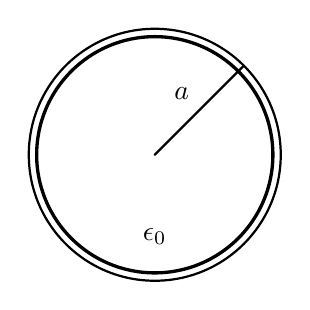
\begin{tikzpicture}
    \draw (0,0) circle (1.6);
    \draw [ very thick ] (0,0) circle (1.5);
    \draw (0,0) node [ below = .8cm ] {$\epsilon_0$} --++ (45:1.6)
     node [ midway, above left ] {$a$};
  \end{tikzpicture}
\end{textfig}
\begin{solution}\leavevmode
  \begin{enumerate}
    \item 由麦克斯韦方程组得
    \[
      \rho = \epsilon_0 \nabla \cdot \bm E
    = \epsilon_0 \frac{1}{r^2} \odv{}r(r^2E)
    = 6\epsilon_0\frac{r^3}{a^4}
    \]
    \item 球内总电荷量
    \[
      Q = \iiint \rho \d V
        = \int_0^a 6\epsilon_0\frac{r^3}{a^4} 4\pi r^2 \d r
        = 4\pi\epsilon_0a^2
    \]
    做半径为 $r$ ($r > a$) 的高斯面，由高斯定理
    \[
      D_1 \cdot 4\pi r^2 = Q + Q = 8\pi\epsilon_0a^2,~ D_1 = 2\epsilon_0a^2/r^2
    \]
    取 $r = a$，此时 $D_1 = 2\epsilon_0$. 同理，做半径为 $r$ ($r < a$) 的高斯面，
    由于球壳内电场为零，所以 $D_2 = 0$. 根据边界条件得外表面电荷密度
    \[\rho_s = D_{n_1} - D_{n_2} = 2\epsilon_0\]
    其中，$D_{n_1} = D_1$，$D_{n_2} = D_2$.
    所以球壳外表面电荷为 $\rho_s \cdot 4\pi a^2 = 2Q$
  \end{enumerate}
\end{solution}

\begin{textfig}[ratio = 3:1]
  \begin{problem}[10 pt]
    半球形导体接地电极，半径为 $a$，大地电导率为 $\sigma$.
    若在接地电极周围半径为 $b$ 的范围内把电导率提高到 $\sigma_1$（例如灌盐水），求接地电阻.
  \end{problem}
  \textfigsplit\centering
  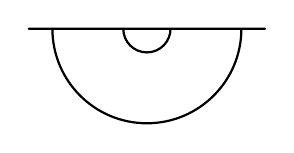
\begin{tikzpicture}
    \draw (-1.5,0) -- (1.5,0) (-1.2,0) arc (-180:0:1.2)
          (-.3,0) arc (-180:0:.3);
  \end{tikzpicture}
\end{textfig}
\begin{solution}
  以接地点为圆心向外辐射的电流密度为
  \[J = I/2\pi r^2\]
  电场强度为
  \[
    E =
    \begin{cases}
      J/\sigma_1 = I/2\pi\sigma_1r^2, & r < a + b\\
      J/\sigma_1 = I/2\pi\sigma r^2, & r > a + b\\
    \end{cases}
  \]
  则接地点的电势为
  \[
    U = \int_a^\infty \bm E \cdot \d\bm r
      = \int_a^b \frac{I}{2\pi\sigma_1 r^2} \cdot \d r +
        \int_b^\infty \frac{I}{2\pi\sigma r^2} \d r
      = \frac{I}{2\pi\sigma_1} \ab(\frac1a - \frac1b) + \frac{I}{2\pi\sigma b}
  \]
  所以接地电阻为 $R = U/I = \frac{1}{2\pi\sigma_1}
    \ab(\frac1a - \frac1b) + \frac{1}{2\pi\sigma b}$.
\end{solution}

\begin{problem}[10 pt]
  $z = 0$ 是两种媒质的分界面. 在 $z > 0$, $\mu_r = 1$, $\bm B = 1.5\hat x + 0.7\hat y + 0.4\hat z\unit\mT$.
  \begin{enumerate}
    \item $z < 0$, $\mu_r = 80$ 时的磁感应强度.
    \item 每个区域的磁化强度和界面磁化面电流密度.
  \end{enumerate}
\end{problem}
\begin{solution}
  \begin{enumerate}
    \item 由磁感应强度法向连续条件 $B_{1_z} = B_{2_z}$ 得 $B_{2_z} = $
  \end{enumerate}
\end{solution}

\begin{problem}[10 pt]
  在空气中，一均匀平面波沿 $\hat y$ 方向传播，其磁场强度的瞬时值表达式
  $\tilde H(y,t) = \hat z \num{4e-4}\cos\ab(\num{e7}\pi t - \beta y + \frac\pi4)\unit{\A/\m}$，试求
  \begin{enumerate}
    \item 相位常数 $\beta$ 和 $t = \qty3\ms$ 时，$H_z = 0$ 的位置.
    \item 求电场强度的瞬时表达式 $\bm E(y,t)$.
  \end{enumerate}
\end{problem}

\tikz
  {
    \begin{scope}
      \clip [ preaction = { draw, ultra thick, DarkGreen },
              preaction = { fill, DarkGreen!5 }, rounded corners = .5em
            ] (-1em,.5em) rectangle (1em,-.5em);
      \fill [ DarkGreen ] (-1em,.5em) rectangle (0,-.5em)
       node [ midway, white ] {\footnotesize \faIcon{question-circle}};
      \node [ font = \small \bfseries \sffamily \color{DarkGreen} ] at (.5em,0) {1};
    \end{scope}
  }

\end{document}